
\documentclass[11pt]{article}

%\setlength\topmargin{-0.1in}
%\setlength\headheight{0in}
%\setlength\headsep{0in}
\setlength\textheight{8.5in}
\setlength\textwidth{6.5in}
\setlength\oddsidemargin{0in}
\setlength\evensidemargin{0in}
\usepackage{placeins}
\usepackage{indentfirst}
\usepackage{amsmath}
\usepackage{graphicx}
\usepackage{listings}
\usepackage{rotating}
\usepackage{subcaption} 
\usepackage{booktabs}
\usepackage{tikz}
\usepackage{fancyhdr}
\usepackage{pdfpages}
\usepackage{hyperref}
\usepackage{longtable}
\usepackage[toc,page]{appendix}
%Glossary
\usepackage[acronym,nonumberlist]{glossaries}
%\glsaddall %includes all acronymns
%Tables
\usepackage{booktabs}
\newcommand{\ra}[1]{\renewcommand{\arraystretch}{#1}}
%Nomenclature
\usepackage{nomencl}
\makenomenclature
\newif\iffirstglossary\firstglossarytrue
%% This removes the main title:
\renewcommand{\nomname}{}
%% this modifies item separation:
\setlength{\nomitemsep}{15pt}
%% this part defines the groups:
%----------------------------------------------
\usepackage{etoolbox}
\renewcommand\nomgroup[1]{%
  \item[\Large\bfseries
  \ifstrequal{#1}{N}{Nomenclature}{%
  \ifstrequal{#1}{A}{List of Abbreviations}{}}%
]\vspace{10pt}} % this is to add vertical space between the groups.
%----------------------------------------------



\pagestyle{fancy}
\usetikzlibrary{shapes,arrows}
\graphicspath{{Figures/}}
\newcommand{\tabitem}{~~\llap{\textbullet}~~}

\newcommand*{\MyIndent}{\hspace*{0.5cm}}%inerts tab in tables



 
\begin{document} 
\pagenumbering{gobble}

	\begin{titlepage}
	\thispagestyle{empty}
		\newcommand{\HRule}{\rule{\linewidth}{0.5mm}}	
		\center
		\LARGE 
		University of Bath\\
	 	Faculty of Engineering \& Design\\[1cm]	
		%textbf{\Large ME30313 Group Business & Design}\\
		\large
		Word count: XXXXX\\[0.5cm]
		{\large\today}\\[1cm]	
		\HRule\\[0.4cm]	
		{\huge\bfseries Systems Modelling \& Simulation Coursework 1}\\[0.4cm] 	
		\HRule\\[1cm]	
		\begin{minipage}{0.4\textwidth}
			\begin{flushleft}
				\large
				\textit{Supervisor}\\
				A. \textsc{Cookson}
			\end{flushleft}
		\end{minipage}
		~
		\begin{minipage}{0.4\textwidth}
			\begin{flushright}
				\large
				\textit{Assessor}\\
				A. \textsc{Cookson} 
			\end{flushright}
		\end{minipage}\\[1.4cm]
		\large
		\textit{Author}\\
		Xavier \textsc{Forde}\\
		\vfill
		\includegraphics[width=0.4\textwidth]{UOB_Logo.png}\\
		\vfill 
	\end{titlepage}

%%% ACRONYMS %%

%%END OF ACRONYMS %%%


\thispagestyle{empty}




\tableofcontents
\thispagestyle{empty}
\listoffigures
\listoftables


\nomenclature[A]{CAD}{Computer Aided Design}


%\printnomenclature


\clearpage
\pagenumbering{arabic}
%\setcounter{page}{1}
\section{Part 1: Software Verification \& Analytical Testing}

\subsection{Quation 1a}
\subsubsection{Derivation of Diffusion Element Matrix}

Here we will derive the 2-by-2 element matrix for a diffusion operator for an arbitrary element $e_{n}$ between the points $x_{0}$ $x_{1}$. The derivation will start from the weak form version of the diffusion integral, after performing integration by parts. This is given by equation \ref{eq:weakform} in the domain $x = 0$ to $x = 1$.

\begin{equation} \label{eq:weakform}
\int_0^1 D \frac{\partial c}{\partial x}  \frac{\partial v}{\partial x}  dx = \int_0^1 vf dx + \left[vD\frac{\partial c}{\partial x} \right]_0^1
\end{equation}

We have the domain from $x = 0$ to $ x = 1$ which we can split into $ne$ number of elements. This is shown pictorially below for the case $ne = 4$.

%Figure to show elements on a line
\begin{figure}[h!]
\centering
\includegraphics[width=0.75\textwidth]{SplitIntoElements.PNG}
\end{figure}

We can now say the integral from $x = 0$ to $x = 1$ is equivalent to the sum of the integral of the individual elements, for the $ne = 4$ case:


%Splitting Intergral into elements
\begin{equation}
\int_0^1 dx = \int_0^\frac{1}{4}  dx + \int_\frac{1}{4}^\frac{2}{4}  dx + \int_\frac{2}{4}^\frac{3}{4}  dx + \int_\frac{3}{4}^1  dx
\end{equation}

To integrate an individual element we will use linear Lagrange nodal basis function \ref{eq:Lagrange} to represent $c$ and $x$, the functions are shown below. The test function $v$ is set to be equal to the basis function $\psi$.

\begin{subequations}
\label{eq:Lagrange}
\begin{align}
c &= c_{0}\psi_{0}(\zeta) + c_1\psi_{1}(\zeta) \label{eq:LagrangeC} \\
x &= x_{0}\psi_{0}(\zeta) + x_1\psi_{1}(\zeta) \label{eq:LagrangeX} \\
v & = \psi_{0} , \psi_{1} \label{eq:LagrangeV} \\
\text{where,}\\
\psi_{0} &= \frac{1 - \zeta}{2} \ \ \ \ ,  \ \ \ \ \psi_{1} = \frac{1 + \zeta}{2} \label{eq:LagrangePSI}\\
\text{and,}\\
\zeta  & = 2 \left(\frac{x - x_0}{x_1 - x_0}\right) - 1 \label{eq:LagrangeZeta}
\end{align}
\end{subequations}
for $x$ in that element between $x_0$ and $x_1$.\\
We need to map the local element to a standard element as shown below. The Jacobian transform $J$ is used to map from the $x$ to the $\zeta$ coordinate system.

%Local element to standard element
\begin{equation} \label{eq:Jacobian}
J = \left \vert \frac{dx}{d\zeta}\right \vert
\end{equation}



%Figure to show elements mapping to standard
\begin{figure}[h!]
\centering
\includegraphics[width=0.75\textwidth]{Local2Standard.PNG}
\end{figure}

Starting with the left hand side of equation \ref{eq:weakform} transforming with the Jacobian to a standard using $dx = Jd\zeta$ we get:

\begin{equation} \label{eq:LHStransform}
\int_{x_0}^{x_{1}} D \frac{\partial c}{\partial x}  \frac{\partial v}{\partial x}  dx =  \int_{-1}^{1} D \frac{\partial c}{\partial x}  \frac{\partial v}{\partial x} J d\zeta
\end{equation}

We need to evaluate the derivatives $\frac{\partial c}{\partial x}$ and $ \frac{\partial v}{\partial x}$ which we can obtain by applying the chain rule to the definitions of c and v given by equations {eq:LagrangeC} and {eq:LagrangeV}. This gives the results

\begin{subequations}
\label{eq:LagrangeD}
\begin{align}
\frac{dc}{dx} &= c_{0}\frac{d\psi_{0}}{d\zeta}\frac{d\zeta}{dx} + c_1\frac{d\psi_{1}}{d\zeta}\frac{d\zeta}{dx} = c_n\frac{d\psi_{n}}{d\zeta}\frac{d\zeta}{dx} \label{eq:LagrangeDC} \ \ \ \text{for} \ n =0,1\\
\frac{dv}{dx} &= \frac{d\psi_{m}}{d\zeta}\frac{d\zeta}{dx} \ \ \ \text{for} \ m =0,1 \label{eq:LagrangeDV} 
\end{align}
\end{subequations}

We can now rewrite equation \ref{eq:LHStransform} as the following, recognising $c$ is independent of $x$ and therefore $\zeta$.
\begin{equation} \label{eq:LHStransform}
 c_n\int_{-1}^{1} D \frac{d\psi_{n}}{d\zeta}\frac{d\zeta}{dx} \frac{d\psi_{m}}{d\zeta}\frac{d\zeta}{dx} J d\zeta
\end{equation}

Knowing that $\frac{d\zeta}{dx} = J^{-1}$ (for $x_1 > x_0$) from equation \ref{eq:Jacobian} and that for a given element $J$ is constant, we can rewrite equation \ref{eq:LHStransform} as

\begin{equation} \label{eq:LHStransform2}
 c_nJ^{-1}\int_{-1}^{1} D \frac{d\psi_{n}}{d\zeta}\frac{d\psi_{m}}{d\zeta} d\zeta \ \ \ \ \text{for} n= 0,1 \& m = 0,1
\end{equation}




From \ref{eq:LHStransform2} we have two equations, one for each node, which when written in full, is clearly suitable for matrix representation.

\begin{subequations}
\label{eq:matrixform}
\begin{align}
&J^{-1} \left  [c_0 \int_{-1}^{1} D \frac{d\psi_{0}}{d\zeta} \frac{d\psi_{0}}{d \zeta} d \zeta + c_1 \int_{-1}^{1} D \frac{d\psi_{1}}{d\zeta} \frac{d\psi_{0}}{d\zeta}d\zeta ) \right ] \label{eq:row1} \\
&J^{-1} \left  [ c_0 \int_{-1}^{1} D \frac{d\psi_{1}}{d\zeta} \frac{d\psi_{0}}{d \zeta} d \zeta + c_1 \int_{-1}^{1} D \frac{d\psi_{1}}{d\zeta} \frac{d\psi_{1}}{d\zeta}d\zeta ) \right ] \label{eq:row2} 
\end{align}
\end{subequations}

The matrix representation is as follows where $I_{nm}$ represents the individual integrals in the above equations \ref{eq:row1} and \ref{eq:row2}. 

%%%	MATRIX Int_nm%%%%%
\begin{equation}
J^{-1}
\begin{bmatrix}

Int_{00} & Int_{01} \\
Int_{10} & Int_{11}
\end{bmatrix}
\begin{bmatrix}

c_{0} \\  c_{1} 
\end{bmatrix}
\end{equation}

%%Evaluate integrals%%%%%%%%%
We now need to evaluate each $Int_{nm}$ term individually. In order to evaluate the integrals we need to calculate the derivatives of $\psi_0$ and $\psi_{1}$ with respect to $\zeta$ using the definition of the basis function given by equation \ref{eq:LagrangePSI}. The results is as follows.

\begin{subequations}
\label{eq:prematrix}
\begin{align}
\frac{d\psi_{0}}{d\zeta} &= \frac{d}{d\zeta}(\frac{1-\zeta}{2}) = -\frac{1}{2} \label{eq:psi0der}\\
\frac{d\psi_{1}}{d\zeta} &= \frac{d}{d\zeta}(\frac{1+\zeta}{2}) = \frac{1}{2} \label{eq:psi1der}
\end{align}
\end{subequations}
\\


\underline{$Int_{00}$} \\


\begin{equation}\label{eq:Int00}
\begin{split}
 Int_{00} &= \int_{-1}^{1} D \frac{d\psi_{0}}{d\zeta} \frac{d\psi_{0}}{d \zeta} d \zeta \\
&=  \int_{-1}^{1} D .( -\frac{1}{2}). (-\frac{1}{2}) d\zeta \\
& = \left[ \frac{D}{4} \zeta \right]_{-1}^{1} \\
& = \left[ (\frac{D}{4}.1) - (\frac{D}{4}.-1) \right] \\
& = \frac{D}{2}
\end{split}
\end{equation}

\underline{$Int_{01}$} \\


\begin{equation}\label{eq:Int01}
\begin{split}
 Int_{01} &= \int_{-1}^{1} D \frac{d\psi_{0}}{d\zeta} \frac{d\psi_{1}}{d \zeta} d \zeta \\
&=  \int_{-1}^{1} D .( -\frac{1}{2}). (\frac{1}{2}) d\zeta \\
& = \left[-\frac{D}{4} \zeta \right]_{-1}^{1} \\
& = \left[ (-\frac{D}{4}.1) - (-\frac{D}{4}.-1) \right] \\
& = -\frac{D}{2}
\end{split}
\end{equation}

\underline{$Int_{10}$} \\


\begin{equation}\label{eq:Int10}
\begin{split}
 Int_{01} &= \int_{-1}^{1} D \frac{d\psi_{1}}{d\zeta} \frac{d\psi_{0}}{d \zeta} d \zeta \\
&=  \int_{-1}^{1} D .( \frac{1}{2}). (-\frac{1}{2}) d\zeta \\
& = \left[-\frac{D}{4} \zeta \right]_{-1}^{1} \\
& = \left[ (-\frac{D}{4}.1) - (-\frac{D}{4}.-1) \right] \\
& = -\frac{D}{2}
\end{split}
\end{equation}


\clearpage

\underline{$Int_{11}$} \\


\begin{equation}\label{eq:Int11}
\begin{split}
 Int_{11} &= \int_{-1}^{1} D \frac{d\psi_{1}}{d\zeta} \frac{d\psi_{1}}{d \zeta} d \zeta \\
&=  \int_{-1}^{1} D .( \frac{1}{2}). (\frac{1}{2}) d\zeta \\
& = \left [\frac{D}{4} \zeta \right ]_{-1}^{1} \\
& = \left [ (\frac{D}{4}.1) - (\frac{D}{4}.-1) \right ] \\
& = \frac{D}{2}
\end{split}
\end{equation}

We can now assemble our local element matrix (not including the c term matrix). This is the form used in the code for LaplaceElemMatrix.m function. Where J and D are scalars (we have assumed D to be constant).

%%%	Final MATRIX Int_nm%%%%%
\begin{equation} \label{eq:diffmatrix}
J^{-1}D
\begin{bmatrix}

0.5 & -0.5 \\
-0.5 & 0.5
\end{bmatrix}
\end{equation}

%%%%PASSING THE UNIT TEST Q1a%%%%%%%%%%%%

\subsubsection{Passes Unit Tests}

Figure \ref{fig:unittest1} shows the function LaplaceElemMatrix.m passes the unit tests defined in CourseworkOneUnitTest.m with no errors.

%Screenshot pass unit test
\begin{figure}[h!]
\centering \label{fig:unittest1}
\includegraphics[width=0.75\textwidth]{CW1Test.PNG}
\end{figure}



\subsection{Question 1b}
\subsubsection{Derivation of Reaction Element Matrix}

We need to calculate the local element matrix for the diffusion term. This is found by evaluating equation \ref{eq:reation1} term from equation XXXX(Overall equation).

\begin{equation} \label{eq:reation1}
\int_{x_{0}}^{x_{1}} \lambda c v  dx
\end{equation}

As in part a we will apply the Jacobi to map to the $\zeta$ domain. This gives us equation \ref{eq:reatJ}.

\begin{equation} \label{eq:reactJ}
\int_{-1}^1 \lambda c v J d\zeta
\end{equation}

We will again use the basis function for $c$ defined by equation \ref{eq:LagrangeC} and the Galerkin assumption to set the weighting to be the same as that of the basis function for optimal convergance as per equation \ref{eq:LagrangeV}. We can then write equation \ref{eq:reactJ} as a set of two equations similar to equations \ref{eq:row1} and \ref{eq:row2}, assuming $\lambda$ to be independent of $x$ we get the following result. These equations can also be written in the form of a matrix as shown by equation \ref{eq:reactunsolvedmatrix}.

\begin{subequations}
\label{eq:reactmatrixform}
\begin{align}
&J \lambda \left  [c_0 \int_{-1}^{1} \psi_{0} \psi_{0} d \zeta + c_1 \int_{-1}^{1} \psi_{1} \psi_{0} d\zeta ) \right ] \label{eq:reactrow1} \\
&J \lambda \left  [c_0 \int_{-1}^{1} \psi_{0} \psi_{1} d \zeta + c_1 \int_{-1}^{1} \psi_{1} \psi_{1} d\zeta ) \right ]  \label{eq:reactrow2} 
\end{align}
\end{subequations}



\begin{equation} \label{eq:reactunsolvedmatrix}
J \lambda
\begin{bmatrix}

Int_{00} & Int_{01} \\
Int_{10} & Int_{11}
\end{bmatrix}
\begin{bmatrix}

c_{0} \\  c_{1} 
\end{bmatrix}
\end{equation}

We shall now evaluate the $Int_{nm}$ integrals to derive the matrix.

\underline{$Int_{00}$} \\
\begin{equation}\label{eq:Int00}
\begin{split}
 Int_{00} &= \int_{-1}^{1} \psi_{0}\psi_{0} \ d \zeta \\
&=  \int_{-1}^{1}  \Big ( \frac{1-\zeta}{2} \Big )^2 d\zeta \\
& = \left[ \frac{1}{3} \Big ( \frac{1-\zeta}{2} \Big )^3 (-2) \right]_{-1}^{1} \\
& = \frac{2}{3}
\end{split}
\end{equation}

\underline{$Int_{01} = Int_{10}$} \\

\begin{equation}\label{eq:Int01}
\begin{split}
 Int_{00} &= \int_{-1}^{1} \psi_{0}\psi_{1} \ d \zeta \\
&=  \int_{-1}^{1}  \Big ( \frac{1-\zeta}{2} \Big )  \Big ( \frac{1+\zeta}{2} \Big )d\zeta \\
& = \left[ \frac{\zeta}{4} - \frac{\zeta^3}{12}\right]_{-1}^{1} \\
& = \left[ \frac{1}{6} -  \Big (-\frac{1}{4} + \frac{1}{12} \Big )\right]_{-1}^{1} \\
& = \frac{1}{3}
\end{split}
\end{equation}

\underline{$Int_{11}$} \\
\begin{equation}\label{eq:Int00}
\begin{split}
 Int_{00} &= \int_{-1}^{1} \psi_{1}\psi_{1} \ d \zeta \\
&=  \int_{-1}^{1}  \Big ( \frac{1+\zeta}{2} \Big )^2 d\zeta \\
& = \left[ \frac{1}{3} \Big ( \frac{1+\zeta}{2}\Big)^3 . 2 \right]_{-1}^{1} \\
& = \frac{2}{3}
\end{split}
\end{equation}

Putting the results of the integrals into the matrix for from equation \ref{eq:reactunsolvedmatrix} we get the result shown by equation \ref{eq:reactmatrix}. This result is used by the LinearReactionElemMatrix.m function. As per equation XXXX we will need to subtract this result from the local diffusion element matrix result given by equation \ref{eq:diffmatrix} in order to get the overall local element matrix which we can then assemble into an global matrix.

%%%	Reaction Matrix%%%%%
\begin{equation} \label{eq:reactmatrix}
J\lambda
\begin{bmatrix}

\frac{2}{3} & \frac{1}{3}  \\[1ex]
 \frac{1}{3}  & \frac{2}{3}
\end{bmatrix}
\end{equation}

\subsubsection{Solving Laplace With Dirichlet Boundaries}

We will use the finite element solver to solve Laplace's equation: 

\begin{equation}
\label{eq:Laplace}
\frac{\partial^2 c}{\partial x^2} = 0
\end{equation}

over the domain $x = 0$ to $x = 1$ with the Dirichlet boundary conditions:

\begin{subequations}\label{eq:LaplaceBCs}
\begin{align}
c = 2 \ \ at \ \ x = 0 \\
c = 0 \ \ at \ \ x  = 1
\end{align}
\end{subequations}

The analytical solution is given by equation \ref{eq:LaplaceAnalytical}.

\begin{equation}\label{eq:LaplaceAnalytical}
c = 2(1-x)
\end{equation}

The result of the analytical solution has been plotted in \ref{fig:LaplaceFig1} with the FEM results overlaid. The FEM solution is very accurate here because we have used linear approximations as our basis functions and the analytical solution is also linear. This means we can achieve good results even with a low resolution 4 element mesh.

\begin{figure}[h!] \label{fig:LaplaceFig1}
    \centering
    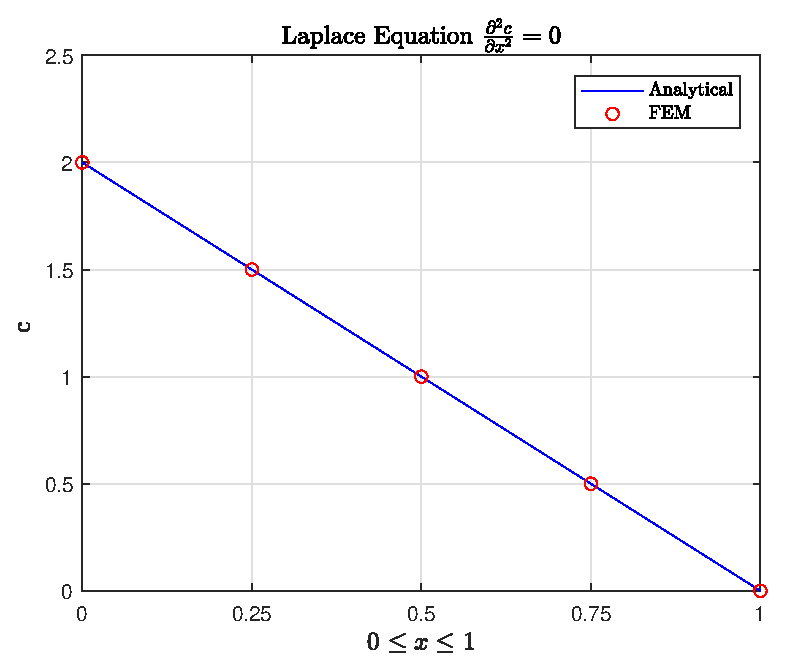
\includegraphics{epsLaplaceFig1}
    \caption{Comparison of Analytical and Finite Element Solutions of Laplace's Equation}
\end{figure}

\subsubsection{Add a Neumann Boundary}
Now we will change the initial boundary condition to a Neumann boundary, the conditions are given by equations \ref{eq:LaplaceBCs2}.

\begin{subequations}\label{eq:LaplaceBCs2}
\begin{align}
\frac{dc}{dx} = 2 \ \ at \ \ x = 0 \\
c = 0 \ \ at \ \  x= 1
\end{align}
\end{subequations}

\begin{figure}[h!] \label{fig:LaplaceFig2}
    \centering
    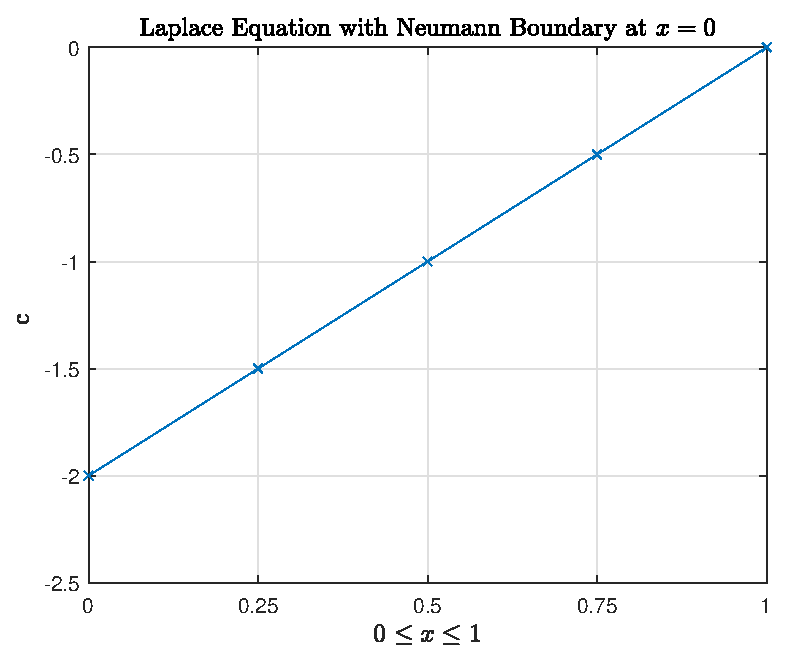
\includegraphics{epsLaplaceFig2}
    \caption{Comparison of Analytical and Finite Element Solutions of Laplace's Equation}
\end{figure}

\section{Part 2}



\pagebreak



%\begin{thebibliography}{9}
%%Last name, First Initial, Year published. Title. Publisher, Volume, Page(s).
%% HARVARD REFERENCE STYLE:
%%Brunner, F.H., 1949. Synthetic gasoline from natural gas. Industrial and engineering chemistry, 41(11), pp.2511-2515.
%
%\bibitem{SPEC} 
%Macgregor, K., 2017. 
%\textit{Student Design Project Specification 2017/18.}
%Airbus Group.


%\end{thebibliography}

%\pagebreak
%
%\begin{appendices}
%\section{Cash Flow Statement}
%
%\begin{figure}[p]  %nrcVrc Figure
%	\centering
%	\includegraphics[width=1.2\textwidth, angle=270]{cashflow1.png}
%\end{figure} 
%
%\begin{figure}[p]  %nrcVrc Figure
%	\centering
%	\includegraphics[width=1.2\textwidth, angle=270]{cashflow2.png}
%\end{figure} 
%
%\pagebreak
%\section{General Arrangement Drawing}
%\end{appendices}





\end{document}

